\documentclass{report}

\usepackage{import}
\import{../}{gov-style}
\addbibresource{../thesis.bib}

\begin{document}
\section{Introduction}
\subsection{In space, no one will shoot you down}
Though each of the six flags on the moon was once an American flag, the United States does not own the moon.\footnote{I say ``was once'' because all of the flags are now bleached white after years of direct exposure to sunlight. (\cite{spudis_faded_2011})} Were China to launch a manned lunar mission tomorrow, and plant their own flag on the surface of the moon, no one would question their right to do so, but no one would interpret that as a claim to ownership either. The history of human activity in space follows that exact pattern. A state has the essentially unquestioned right to put anything in space, so long as it does not interfere with anything that another state has already placed there. The Outer Space Treaty (OST), which entered into force only ten years after \emph{Sputnik}, formalized this practice: ``Outer space \textelp{} is not subject to national appropriation by claim of sovereignty, by means of use or occupation, or by any other means.''\footcite{noauthor_outer_1966} The strength of the OST has never been tested. Not once in the history of human space activity have hostile forces disabled, damaged, or destroyed an object in space that was not their own.

While it makes perfect sense that no state has attempted to enforce a territorial claim on the moon---technological feasibility aside, there's not much up there---artificial satellites present a much more tempting target. Satellites are numerous, accessible, and undergird essential civil infrastructure. That such an equilibrium held throughout the Cold War---in which all satellites, regardless of their applicability to military, commercial, or scientific ends, were left undisturbed---is one of the most remarkable achievements of the international system. The world today relies on communication infrastructure that only exists because the safety of the satellites that make them possible is functionally guaranteed by decades of peace in outer space.

Why was the USSR comfortable shooting down aircraft manned by uniformed Air Force officers, but not a small instrument of extraterrestrial espionage? The untouchable nature of satellites marks the most successful iteration of the intelligence norms that have been discussed in this thesis so far. While Cold War norms limit the diplomatic response to reconnaissance flights and human espionage, they cannot eliminate the response entirely, because those activities run afoul of longstanding principles regarding territorial integrity and domestic law. In space, where no such principles exist, the only established norm at the dawn of the space age was one from the world of espionage---that intelligence-gathering entities are not inherently aggressive. Thus space became an environment where a strike against a satellite would constitute the first act of aggression, even though the satellite was potentially gathering information that could significantly compromise a state's security position.

In this chapter I will interrogate how the norm against using anti-satellite (ASAT) weapons has held for over 60 years. Unlike in previous chapters, it is not necessary to prove that there is a muted diplomatic response to spying from a satellite because the lack of response is self-evident---no nation has ever challenged the right of another to launch a satellite, and even when concerns about their espionage utility have been raised, those concerns never resulted in military action. The first section will demonstrate how Eisenhower designed the rollout of the American satellite program with an eye towards influencing international law, developing a norm that would permit reconnaissance satellites. The following section will examine how the norm preserving intelligence capabilities was a significant factor in preventing the weaponization of space during the 1980s. And the final section discusses how well that norm is performing today.

\section{How Eisenhower legitimized reconnaissance satellites}
\subsection{The spy plane walked so the spy satellite could run}
Well before the \emph{Sputnik} launch, the Eisenhower administration realized that a satellite might able to consistently perform the photo-reconnaissance overflight that a spy plane never could. In the later half of the 1950s, the U-2 flew high enough to avoid Soviet anti-aircraft capabilities, but that status quo had a clear expiration date. The Soviet Union made it clear that they were annoyed by the overflights, and continued to register diplomatic protests about them. Eventually the Soviets would be able to able to shoot a U-2 craft down, and because it gathered strategic intelligence in clear violation of Soviet territorial airspace, they would been well within their rights to do so---which is exactly what happened in 1960.

Theoretically, the exact same dynamic could have played out a with the development of spy satellites: the US develops a new photo-reconnaissance technology which its main adversary is unable to prevent; the USSR diplomatically objects to the technology's use; the USSR finally develops a weapon capable of counteracting the new technology; and the USSR employs it. Each one of these steps came to pass except the last---even after developing a feasible ASAT weapon, the Soviet Union never made use of it. And the onus was on them to push back against the American efforts to normalize satellite reconnaissance. \emph{Sputnik} briefly put the USSR at the forefront of the final frontier, but the satellite itself was totally innocuous; it obtained data about the density of the atmosphere and propagation of radio waves.\footcite{nasa_sputnik_2019} It was the United States that would first launch a satellite capable of photo-reconnaissance---and it was the Soviet Union that would let them get away with it.

The international legal regime that decided non-weaponized satellites were ``peaceful'' was never a foregone conclusion. The norm against ASAT strikes was a deliberate product of Eisenhower's foreign policy, the primary goal of which was to gain access to the closed Soviet state via photo-reconnaissance.\footcite[p.~65]{hayes_struggling_1994} In 1954, the same year that he approved Project AQUATONE, Eisenhower convened the Office of Defense Mobilization's Science Advisory Committee. Chaired by MIT President Dr. James Killian, the Science Advisory Committee was tasked with divining technical solutions to mitigate the threat of a nuclear Pearl Harbor.\footcite[p.~115]{mcdougall_heavens_1985} From their work resulted the Technological Capabilities Panel (TCP) Report---formally titled ``Meeting the Threat of a Surprise Attack,'' but also variously referred to as the ``Killian Report,'' ``TCP Report,'' or ``Surprise Attack Study.'' It predicted that four distinct periods of relative power would unfold over the next decade, starting with the current era in which neither side was capable of a decisive strike but the US had a relative advantage in air-atomic power, and ending in a world where mutual ICBM capabilities ensured that the balance of power would remain a stalemate indefinitely.\footcite[p.~116]{mcdougall_heavens_1985}

All four Cold War phases that the Killian Report predicted---with shocking accuracy, as it turned out---had one thing in common: the sobering analysis that a great power conflict would result in heavy American losses. Even in the phase where American relative power was to be at its greatest, before the development of Soviet multimegaton capability, the United States ``would be severely damaged,'' and ``emerge a battered victor'' in the event of a surprise attack.\footcite{technological_capabilities_panel_meeting_1955} Killian wrote that, while presenting the report to the NSC, ``we emphasized that even though our \emph{relative} military strength might change in the manner suggested in the table, we still would be in a position where the United States could be grievously hurt.''\footcite[p.~75]{killian_sputnik_1977} Therefore, it was imperative that the United States be able to anticipate a surprise attack, but also avoid starting a conflict in the event of a false positive. ``We \emph{must} find ways to increase the number of hard facts upon which our intelligence estimates are based,'' the report states, ``to provide better strategic warning, to minimize surprise in the kind of attack, and to reduce the danger of gross overestimation or gross underestimation of the threat.''\footcite{technological_capabilities_panel_meeting_1955}



The first document ... was 1950

Everything about the administration's satellite policy was designed to set the stage for the eventual launch of a spy satellite, which they achieved by not launching spy satellites right way.

The norm establishing that offensive ASAT attacks are off-limits has over 60 years of empirical force behind it, but when \emph{Sputnik} launched in 1957, the safety of artificial satellites was far from guaranteed. The Eisenhower administration purposefully designed its satellite program so that it would establish a norm of peaceful development within the blank slate of international space law. The desired effect was to legitimize a particular type of satellite---a reconnaissance satellite that could fly over Soviet airspace with impunity, and finally grant Eisenhower the effect of an Open Skies policy which Khrushchev had previously rebuffed. The administration's success resulted in a norm against shooting down satellites.

Intelligence norms formed space norms, not the other way around. That every type of satellite is free from the threat of weapons is a byproduct of the intelligence norms that legitimized the use of spy satellites.

\section{Reagan, Star Wars, and the fervor of space weaponization}
That peace is all the more remarkable when you consider that even though space has never been weaponized, it has been thoroughly \emph{militarized}. The difference between the two is significant; weaponization requires the placement of space-based devices that have destructive capacity, such as an orbital satellite loaded with nuclear bombs, while militarization is simply the use of space-based devices to facilitate military operations.\footcite[p.~3]{mowthorpe_militarization_2004} Currently no one faces the threat of an attack originating from space, but an incredible number of more traditional American military capabilities rely on the network of satellites. According to the official government website, The Global Positioning System (GPS) alone is used by the DoD for precision guided munition strikes, force tracking, search and rescue, and remote piloting of unmanned aerial vehicles.\footcite{national_coordination_office_for_space-based_positioning_navigation_and_timing_federal_2018} A fleet of spy satellites, built and maintained by the National Reconnaissance Office since 1961, take high-resolution photos of places Gary Powers could never have reached.\footcite{national_reconnaissance_office_about_2019} The many commercial and civil satellites operated by American entities have military applications as well.

The question of why space has been peacefully militarized but never weaponized is one that this thesis will mostly sidestep. The academic literature on space weaponization was briefly hijacked when Ronald Reagan announced the Strategic Defense Initiative (SDI) on March 23, 1983. Derisively nicknamed ``Star Wars,'' the core promise of the SDI was that, with an Apollo-style research effort, the United States would be able to develop an effective way to end the threat of ballistic nuclear missiles.\footcite{reagan_address_1983} The SDI and the Reagan administration's renewed interest in space conflict overwhelmed the policy research sphere, which was soon consumed with analyzing how best to manage a battlefield that was entirely theoretical, and, to a degree not understood at the time, technologically infeasible. Scholarly work on space policy quickly responded to the possibilities of a world where dueling superpowers were equipped with space-based X-ray lasers, particle beams, and kinetic ballistic missile interceptors---a world which did not exist then, and still belongs to science fiction today.\footcite[p.~1-2]{moorhead_work_2013}

Instead, I am concerned with one specific type of space weapon, far more pedestrian than space lasers, but also technologically feasible, successfully tested, virtually unregulated, and potentially catastrophic. A strategic first-strike against American satellites carries the potential to cripple the United States military's intelligence, communications, and ballistics capabilities, to say nothing of the effect on civil society as televisions go dark and cell phones lose signal. Such a strike is made by possible by anti-satellite (ASAT) weapons---and such a strike has remarkably never been executed.


\section{Satellites today}
There are a lot of possible targets.\footcite[A few satellites are listed as dual-purpose (i.e. Government/Military), and those are counted twice, once for each purpose. For instance, the data shows that the US is currently operating 830 satellites, while adding up the bars in this chart would give you 966. I made this choice to emphasize the dependency of various social systems on the existing satellite infrastructure.]{union_of_concerned_scientists_ucs_2018}


\begin{figure}[ht]
  \centering
  % Created by tikzDevice version 0.12 on 2019-05-03 23:25:55
% !TEX encoding = UTF-8 Unicode
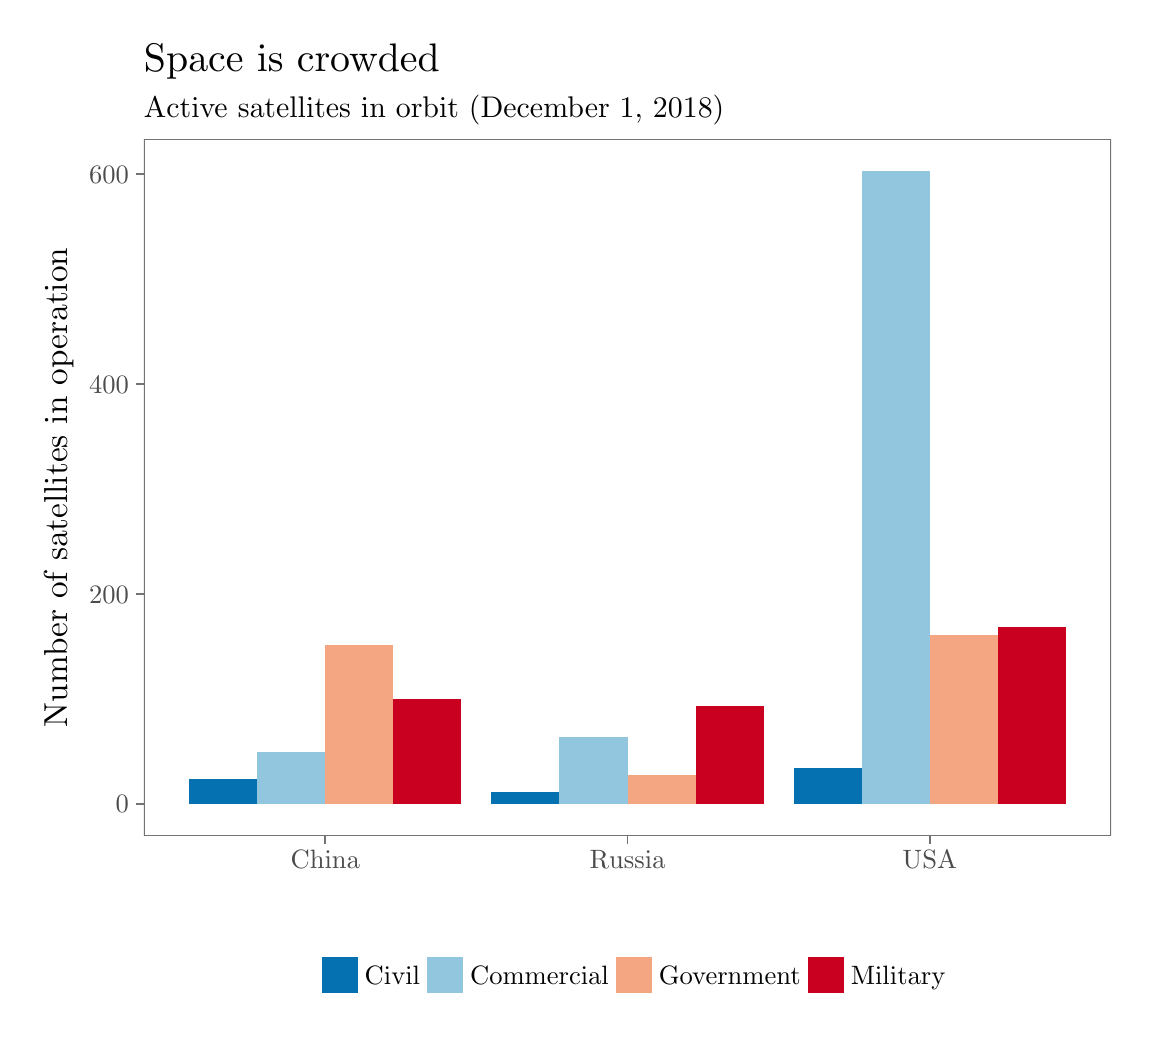
\begin{tikzpicture}[x=1pt,y=1pt]
\definecolor{fillColor}{RGB}{255,255,255}
\path[use as bounding box,fill=fillColor,fill opacity=0.00] (0,0) rectangle (397.48,361.35);
\begin{scope}
\path[clip] (  0.00,  0.00) rectangle (397.48,361.35);
\definecolor{drawColor}{RGB}{255,255,255}
\definecolor{fillColor}{RGB}{255,255,255}

\path[draw=drawColor,line width= 0.6pt,line join=round,line cap=round,fill=fillColor] (  0.00,  0.00) rectangle (397.48,361.35);
\end{scope}
\begin{scope}
\path[clip] ( 42.01, 69.49) rectangle (391.48,320.95);
\definecolor{fillColor}{RGB}{255,255,255}

\path[fill=fillColor] ( 42.01, 69.49) rectangle (391.48,320.95);
\definecolor{fillColor}{RGB}{202,0,32}

\path[fill=fillColor] (132.11, 80.92) rectangle (156.68,118.83);
\definecolor{fillColor}{RGB}{244,165,130}

\path[fill=fillColor] (107.53, 80.92) rectangle (132.11,138.17);
\definecolor{fillColor}{RGB}{146,197,222}

\path[fill=fillColor] ( 82.96, 80.92) rectangle (107.53, 99.50);
\definecolor{fillColor}{RGB}{5,113,176}

\path[fill=fillColor] ( 58.39, 80.92) rectangle ( 82.96, 90.02);
\definecolor{fillColor}{RGB}{202,0,32}

\path[fill=fillColor] (241.32, 80.92) rectangle (265.89,116.18);
\definecolor{fillColor}{RGB}{244,165,130}

\path[fill=fillColor] (216.75, 80.92) rectangle (241.32, 91.16);
\definecolor{fillColor}{RGB}{146,197,222}

\path[fill=fillColor] (192.17, 80.92) rectangle (216.75,105.19);
\definecolor{fillColor}{RGB}{5,113,176}

\path[fill=fillColor] (167.60, 80.92) rectangle (192.17, 85.09);
\definecolor{fillColor}{RGB}{202,0,32}

\path[fill=fillColor] (350.53, 80.92) rectangle (375.10,144.61);
\definecolor{fillColor}{RGB}{244,165,130}

\path[fill=fillColor] (325.96, 80.92) rectangle (350.53,141.96);
\definecolor{fillColor}{RGB}{146,197,222}

\path[fill=fillColor] (301.38, 80.92) rectangle (325.96,309.52);
\definecolor{fillColor}{RGB}{5,113,176}

\path[fill=fillColor] (276.81, 80.92) rectangle (301.38, 93.81);
\definecolor{drawColor}{gray}{0.45}

\path[draw=drawColor,line width= 0.6pt,line join=round,line cap=round] ( 42.01, 69.49) rectangle (391.48,320.95);
\end{scope}
\begin{scope}
\path[clip] (  0.00,  0.00) rectangle (397.48,361.35);
\definecolor{drawColor}{gray}{0.30}

\node[text=drawColor,anchor=base east,inner sep=0pt, outer sep=0pt, scale=  0.96] at ( 36.61, 77.62) {0};

\node[text=drawColor,anchor=base east,inner sep=0pt, outer sep=0pt, scale=  0.96] at ( 36.61,153.44) {200};

\node[text=drawColor,anchor=base east,inner sep=0pt, outer sep=0pt, scale=  0.96] at ( 36.61,229.26) {400};

\node[text=drawColor,anchor=base east,inner sep=0pt, outer sep=0pt, scale=  0.96] at ( 36.61,305.08) {600};
\end{scope}
\begin{scope}
\path[clip] (  0.00,  0.00) rectangle (397.48,361.35);
\definecolor{drawColor}{gray}{0.45}

\path[draw=drawColor,line width= 0.6pt,line join=round] ( 39.01, 80.92) --
	( 42.01, 80.92);

\path[draw=drawColor,line width= 0.6pt,line join=round] ( 39.01,156.74) --
	( 42.01,156.74);

\path[draw=drawColor,line width= 0.6pt,line join=round] ( 39.01,232.56) --
	( 42.01,232.56);

\path[draw=drawColor,line width= 0.6pt,line join=round] ( 39.01,308.38) --
	( 42.01,308.38);
\end{scope}
\begin{scope}
\path[clip] (  0.00,  0.00) rectangle (397.48,361.35);
\definecolor{drawColor}{gray}{0.45}

\path[draw=drawColor,line width= 0.6pt,line join=round] (107.53, 66.49) --
	(107.53, 69.49);

\path[draw=drawColor,line width= 0.6pt,line join=round] (216.75, 66.49) --
	(216.75, 69.49);

\path[draw=drawColor,line width= 0.6pt,line join=round] (325.96, 66.49) --
	(325.96, 69.49);
\end{scope}
\begin{scope}
\path[clip] (  0.00,  0.00) rectangle (397.48,361.35);
\definecolor{drawColor}{gray}{0.30}

\node[text=drawColor,anchor=base,inner sep=0pt, outer sep=0pt, scale=  0.96] at (107.53, 57.48) {China};

\node[text=drawColor,anchor=base,inner sep=0pt, outer sep=0pt, scale=  0.96] at (216.75, 57.48) {Russia};

\node[text=drawColor,anchor=base,inner sep=0pt, outer sep=0pt, scale=  0.96] at (325.96, 57.48) {USA};
\end{scope}
\begin{scope}
\path[clip] (  0.00,  0.00) rectangle (397.48,361.35);
\definecolor{drawColor}{RGB}{1,2,2}

\node[text=drawColor,rotate= 90.00,anchor=base,inner sep=0pt, outer sep=0pt, scale=  1.20] at ( 14.26,195.22) {Number of satellites in operation};
\end{scope}
\begin{scope}
\path[clip] (  0.00,  0.00) rectangle (397.48,361.35);
\definecolor{fillColor}{RGB}{255,255,255}

\path[fill=fillColor] ( 96.23,  6.00) rectangle (337.26, 31.84);
\end{scope}
\begin{scope}
\path[clip] (  0.00,  0.00) rectangle (397.48,361.35);
\definecolor{fillColor}{RGB}{255,255,255}

\path[fill=fillColor] (105.53, 11.69) rectangle (119.99, 26.14);
\end{scope}
\begin{scope}
\path[clip] (  0.00,  0.00) rectangle (397.48,361.35);
\definecolor{fillColor}{RGB}{5,113,176}

\path[fill=fillColor] (106.24, 12.40) rectangle (119.27, 25.43);
\end{scope}
\begin{scope}
\path[clip] (  0.00,  0.00) rectangle (397.48,361.35);
\definecolor{fillColor}{RGB}{255,255,255}

\path[fill=fillColor] (143.59, 11.69) rectangle (158.05, 26.14);
\end{scope}
\begin{scope}
\path[clip] (  0.00,  0.00) rectangle (397.48,361.35);
\definecolor{fillColor}{RGB}{146,197,222}

\path[fill=fillColor] (144.31, 12.40) rectangle (157.34, 25.43);
\end{scope}
\begin{scope}
\path[clip] (  0.00,  0.00) rectangle (397.48,361.35);
\definecolor{fillColor}{RGB}{255,255,255}

\path[fill=fillColor] (211.81, 11.69) rectangle (226.26, 26.14);
\end{scope}
\begin{scope}
\path[clip] (  0.00,  0.00) rectangle (397.48,361.35);
\definecolor{fillColor}{RGB}{244,165,130}

\path[fill=fillColor] (212.52, 12.40) rectangle (225.55, 25.43);
\end{scope}
\begin{scope}
\path[clip] (  0.00,  0.00) rectangle (397.48,361.35);
\definecolor{fillColor}{RGB}{255,255,255}

\path[fill=fillColor] (281.16, 11.69) rectangle (295.61, 26.14);
\end{scope}
\begin{scope}
\path[clip] (  0.00,  0.00) rectangle (397.48,361.35);
\definecolor{fillColor}{RGB}{202,0,32}

\path[fill=fillColor] (281.87, 12.40) rectangle (294.90, 25.43);
\end{scope}
\begin{scope}
\path[clip] (  0.00,  0.00) rectangle (397.48,361.35);
\definecolor{drawColor}{RGB}{1,2,2}

\node[text=drawColor,anchor=base west,inner sep=0pt, outer sep=0pt, scale=  0.96] at (121.79, 15.61) {Civil};
\end{scope}
\begin{scope}
\path[clip] (  0.00,  0.00) rectangle (397.48,361.35);
\definecolor{drawColor}{RGB}{1,2,2}

\node[text=drawColor,anchor=base west,inner sep=0pt, outer sep=0pt, scale=  0.96] at (159.86, 15.61) {Commercial};
\end{scope}
\begin{scope}
\path[clip] (  0.00,  0.00) rectangle (397.48,361.35);
\definecolor{drawColor}{RGB}{1,2,2}

\node[text=drawColor,anchor=base west,inner sep=0pt, outer sep=0pt, scale=  0.96] at (228.07, 15.61) {Government};
\end{scope}
\begin{scope}
\path[clip] (  0.00,  0.00) rectangle (397.48,361.35);
\definecolor{drawColor}{RGB}{1,2,2}

\node[text=drawColor,anchor=base west,inner sep=0pt, outer sep=0pt, scale=  0.96] at (297.42, 15.61) {Military};
\end{scope}
\begin{scope}
\path[clip] (  0.00,  0.00) rectangle (397.48,361.35);
\definecolor{drawColor}{RGB}{1,2,2}

\node[text=drawColor,anchor=base west,inner sep=0pt, outer sep=0pt, scale=  1.08] at ( 42.01,328.85) {Active satellites in orbit (December 1, 2018)};
\end{scope}
\begin{scope}
\path[clip] (  0.00,  0.00) rectangle (397.48,361.35);
\definecolor{drawColor}{RGB}{1,2,2}

\node[text=drawColor,anchor=base west,inner sep=0pt, outer sep=0pt, scale=  1.44] at ( 42.01,345.43) {Space is crowded};
\end{scope}
\end{tikzpicture}

  \label{country_sats}
  \caption{Active satellites, grouped by operating country and purpose}
\end{figure}

\newpage
\printbibliography[heading=subbibliography]

\end{document}
